% Arquivo LaTeX de exemplo de dissertação/tese a ser apresentados à CPG
% do IME-USP
% 
% Versão 3: Thu Dec 10 23:57:33 BRST 2009

%
% Criação: Jesús P. Mena-Chalco
% Revisão: Fábio Kon
%  
% Obs: Leia previamente o texto do arquivo README.txt
%

\documentclass[11pt,twoside,a4paper]{book}

% ---------------------------------------------------------------------------- %
% Pacotes 
\usepackage[T1]{fontenc}
\usepackage[brazil]{babel}
\usepackage[utf8]{inputenc}
\usepackage[pdftex]{graphicx}           % usamos arquivos pdf/png como figuras
\usepackage{pifont}
\usepackage{amsfonts}
\usepackage{amssymb} 
\usepackage{setspace}                   % espaçamento flexível
\usepackage[bf,small,compact]{titlesec} % cabeçalhos dos títulos: menores e compactos
\usepackage{indentfirst}                % indentação do primeiro parágrafo
\usepackage{subfigure}                  % uso de várias figuras numa só
\usepackage{makeidx}                    % índice remissivo
\usepackage[nottoc]{tocbibind}          % acrescentamos a bibliografia/indice/conteudo no Table of Contents
\usepackage{courier}                    % usa o Adobe Courier no lugar de Computer Modern Typewriter
\usepackage{type1cm}                    % fontes realmente escaláveis
\usepackage{listings}                   % para formatar código-fonte (ex. em Java)
\usepackage{setspace}
\usepackage{longtable}
\usepackage{multirow}
\usepackage{titletoc}
\usepackage{lscape}
\usepackage[fixlanguage]{babelbib}
\usepackage[font=small,format=plain,labelfont=bf,up,textfont=it,up]{caption}
\usepackage[usenames,svgnames,dvipsnames,table]{xcolor}
\usepackage[a4paper,top=2.54cm,bottom=2.0cm,left=2.0cm,right=2.54cm]{geometry} % margens
\usepackage[pdftex,plainpages=false,pdfpagelabels,pagebackref,colorlinks=true,citecolor=black,linkcolor=black,urlcolor=black,filecolor=black,bookmarksopen=true]{hyperref} % links em preto
%\usepackage[pdftex,plainpages=false,pdfpagelabels,pagebackref,colorlinks=true,citecolor=DarkGreen,linkcolor=NavyBlue,urlcolor=DarkRed,filecolor=green,bookmarksopen=true]{hyperref} % links coloridos
\usepackage[all]{hypcap}                % soluciona o problema com o hyperref e capitulos
\usepackage[numbers,square,sort,nonamebreak,comma]{natbib}  % citação
                                % bibliográfica alpha (alpha-ime.bst)
\usepackage{float}

\usepackage{type1cm}      % fontes realmente escaláveis
\fontsize{60}{62}\usefont{OT1}{cmr}{m}{n}{\selectfont}

% ---------------------------------------------------------------------------- %
\floatstyle{boxed}
\newfloat{caixa}{htb}{bx}
\floatname{caixa}{Caixa}

% ---------------------------------------------------------------------------- %
% headers similares oa TAOP de Donald E. Knuth
\usepackage{fancyhdr}
\pagestyle{fancy}
\fancyhf{}
\renewcommand{\chaptermark}[1]{\markboth{\MakeUppercase{#1}}{}}
\renewcommand{\sectionmark}[1]{\markright{\MakeUppercase{#1}}{}}
\renewcommand{\headrulewidth}{0pt}

% ---------------------------------------------------------------------------- %
\graphicspath{{./figuras/}}             % path das figuras (recomendável)
\frenchspacing                          % Arruma o espaço: id est (i.e.) e exempli gratia (e.g.) 
\urlstyle{same}                         % URL com o mesmo estilo do texto e nao mono-spaced
\makeindex                              % para o índice remissivo
\raggedbottom                           % para não permitir espaços extra no texto
\fontsize{60}{62}\usefont{OT1}{cmr}{m}{n}{\selectfont}
\cleardoublepage
\normalsize

% ---------------------------------------------------------------------------- %
% Opções de listing usados para o código fonte
% Ref: http://en.wikibooks.org/wiki/LaTeX/Packages/Listings
\lstset{ %
language=Java,                  % choose the language of the code
basicstyle=\footnotesize,       % the size of the fonts that are used for the code
numbers=left,                   % where to put the line-numbers
numberstyle=\footnotesize,      % the size of the fonts that are used for the line-numbers
stepnumber=1,                   % the step between two line-numbers. If it's 1 each line will be numbered
numbersep=5pt,                  % how far the line-numbers are from the code
showspaces=false,               % show spaces adding particular underscores
showstringspaces=false,         % underline spaces within strings
showtabs=false,                 % show tabs within strings adding particular underscores
frame=single,	                % adds a frame around the code
framerule=0.6pt,
tabsize=2,	                    % sets default tabsize to 2 spaces
captionpos=b,                   % sets the caption-position to bottom
breaklines=true,                % sets automatic line breaking
breakatwhitespace=false,        % sets if automatic breaks should only happen at whitespace
escapeinside={\%*}{*)},         % if you want to add a comment within your code
backgroundcolor=\color[rgb]{1.0,1.0,1.0}, % choose the background color.
rulecolor=\color[rgb]{0.8,0.8,0.8},
extendedchars=true,
xleftmargin=10pt,
xrightmargin=10pt,
framexleftmargin=10pt,
framexrightmargin=10pt
}

% ---------------------------------------------------------------------------- %
% Corpo do texto
\begin{document}
\frontmatter 
% headers para as páginas do frontmatter 
\fancyhead[RO]{{\footnotesize\rightmark}\hspace{2em}\thepage}
\setcounter{tocdepth}{2}
\fancyhead[LE]{\thepage\hspace{2em}\footnotesize{\leftmark}}
\fancyhead[RE,LO]{}
\fancyhead[RO]{{\footnotesize\rightmark}\hspace{2em}\thepage}

\onehalfspacing  % espaçamento


% ---------------------------------------------------------------------------- %
% Capa
\thispagestyle{empty}
\begin{center}
  \vspace*{2.3cm}
  \textbf{\Large{Métodos ágeis e software livre:\\
      Um estudo do relacionamento entre\\
    estas duas comunidades}}\\
	
  \vspace*{1.2cm} \Large{Hugo Corbucci}
    
  \vskip 2cm \textsc{
    Dissertação apresentada\\[-0.25cm]
    ao\\[-0.25cm]
    Instituto de Matemática e Estatística\\[-0.25cm]
    da\\[-0.25cm]
    Universidade de São Paulo}
    
  \vskip 1.5cm
  Programa: Mestrado em Ciência da Computação\\
  Orientador: Prof. Dr. Alfredo Goldman

  \vskip 1cm \normalsize{Durante o desenvolvimento deste trabalho o
    autor recebeu auxílio financeiro do projeto Qualipso}
	
  \vskip 0.5cm \normalsize{São Paulo, Janeiro de 2010}
\end{center}

% ---------------------------------------------------------------------------- %
% Página de rosto (só para a versão final) \newpage
% \thispagestyle{empty}
%	\begin{center}
%   \vspace*{2.3 cm}
%   \textbf{\Large{Título do trabalho a ser apresentado à \\
%       CPG para a dissertação/tese}}\\
%   \vspace*{2 cm}
%	\end{center}
%
%	\vskip 2cm
%
%	\begin{flushright}
%   Este exemplar corresponde à redação\\
%   final da dissertação devidamente corrigida\\
%   e defendida por Hugo Corbucci\\
%   e aprovada pela Comissão Julgadora.  \vskip 2cm
%
%	\end{flushright}
%	\vskip 4.2cm
%
%	\begin{quote}
%   \noindent Banca Examinadora:
%	
%   \begin{itemize}
%   \item Prof. Dr. Alfredo Goldman (orientador) - IME-USP.
%   \item Prof. Dr. Fabio Kon - IME-USP.
%   \item Prof. Dr. José Carlos Maldonado - ICMC-USP.
%   \end{itemize}
%	  
%	\end{quote}
% \pagebreak

\pagenumbering{roman} % começamos a numerar

% ---------------------------------------------------------------------------- %
% Agradecimentos
\chapter*{Agradecimentos}

Este trabalho contou com o apoio do projeto Qualipso \cite{Qualipso}.

Gostaria de agradecer ao Christian Reis por sua ajuda, pelas
discussões interessantes e pelo apoio. Aos meus pais, pela confiança e
pelo apoio. À Mariana Bravo pelo apoio, companhia, revisões e ajudas
constantes ao longo de todo esse tempo. Ao Danilo Sato e Daniel
Cordeiro pelas revisões e críticas ao texto além das excelentes
discussões. Aos outros membros da AgilCoop pelas experiências, ideias,
conversas e ajudas.
% TODO Completar

% ---------------------------------------------------------------------------- %
% Resumo
\chapter*{Resumo}

A relação entre métodos ágeis e software livre é, no mínimo,
indefinida. A princípio, as duas comunidades não parecem ter nenhuma
relação já que uma representa uma família de metodologias de
desenvolvimento de software e a outra, uma forma de licenciar código
fonte de um projeto. Observando com um pouco mais de cuidado
percebe-se que as comunidades compartilham diversas práticas e,
aparentemente, as motivações para aplicar tais práticas são
semelhantes. Esse trabalho estuda essa relação mais a fundo e
apresenta semelhanças e diferenças entre as duas comunidades. A partir
disso, espera-se facilitar a identificação das soluções de cada
comunidade e contribuir com sugestões de ferramentas e processos de
desenvolvimento em ambos ambientes.

\noindent \textbf{Palavras-chave:} métodos ágeis, open source,
software livre

% ---------------------------------------------------------------------------- %
% Abstract
\chapter*{Abstract}

The relationship between agile methods and open source software is, at
least, undefined. At first glance, the two communities do not seem to
have any relationship since one represents a family of software
development methodologies and the other, a way to license a project's
source code. With a more careful observation one can notice that the
communities share several practices and appear to be motivated by the
same reasons. This work studies this relationship more deeply and
presents similarities and differences between the two
communities. This result should help to identify the solutions of
each community and contribute with suggestions of development tools
and processes in both environments.

\noindent \textbf{Keywords:} agile methods, open source, free software

% ---------------------------------------------------------------------------- %
% Sumário
\tableofcontents % imprime o sumário

% ---------------------------------------------------------------------------- %
% Listas: abreviaturas, símbolos, figuras e tabelas

\chapter{Lista de Abreviaturas}
\begin{tabular}{ll}
  SL       & Software Livre.\\
  OSS         & Software de Código Aberto (\emph{Open Source
    Software}).\\
  XP       & Programação Extrema (\emph{Extreme Programming}).\\
  FLOSS       & Software Gratuito, Livre e de Código Aberto
  (\emph{Free, Libre and Open Source Software}).\\
  TDD       & Desenvolvimento Dirigido por Teste
  (\emph{Test Driven Development}).\\
  BDD       & Desenvolvimento Dirigido por Comportamento
  (\emph{Behaviour Driven Development}).\\
  IRC       & Papo Retransmitido pela Internet (\emph{Internet Relay
    Chat}).\\
  FISL       & Fórum Internacional de Software Livre.\\
  API       & Interface de Programação da Aplicação (\emph{Application
    Programming Interface}).\\
  OMM       & Modelo de Maturidade para Software Livre (\emph{Open
    Source Maturity Model}).\\
  CMM       & Modelo de Maturidade de Capabilidade (\emph{Capability
    Maturity Model}).\\
  SEI       & Instituto de Engenharia de Software (\emph{Software
    Engineering Institute}).\\
\end{tabular}

% \chapter{Lista de Símbolos}
% \begin{tabular}{ll}
%		$\omega$    & Freqüência angular.\\
%\end{tabular}

\listoffigures % lista de Figuras
%\listoftables % lista de Tabelas

% ---------------------------------------------------------------------------- %
% Capítulos
\mainmatter
% cabecalho para as páginas do 'mainmatter'
\fancyhead[RE,LO]{\thesection}

% \singlespacing % espaçamento simples
\onehalfspacing % espaçamento um e meio
% \doublespacing % espaçamento duplo

\input cap-introducao % associado ao arquivo: 'cap-introducao.tex'
\input cap-escopo % associado ao arquivo: 'cap-escopo.tex'
\input cap-semelhancas % associado ao arquivo: 'cap-semelhancas.tex'
\input cap-pesquisas % associado ao arquivo: 'cap-pesquisas.tex'
\input cap-diferencas % associado ao arquivo: 'cap-diferencas.tex'
\input cap-omm % associado ao arquivo: 'cap-omm.tex'
\input cap-conclusoes % associado ao arquivo: 'cap-conclusoes.tex'

% cabecalho para os apêndices
\renewcommand{\chaptermark}[1]{\markboth{\MakeUppercase{\appendixname\ \thechapter}} {\MakeUppercase{#1}} }
\fancyhead[RE,LO]{}
\appendix

\chapter{Pesquisa realizada no Encontro Ágil 2008}
\label{ape:EA}

A pesquisa apresentada na Figura \ref{fig:pesquisaEA} foi impressa em
papel e distribuída junto com o material do
evento\footnote{http://www.encontroagil.com.br/ - Último acesso
  27/04/2009} .

\begin{figure}[th]
  \centering
  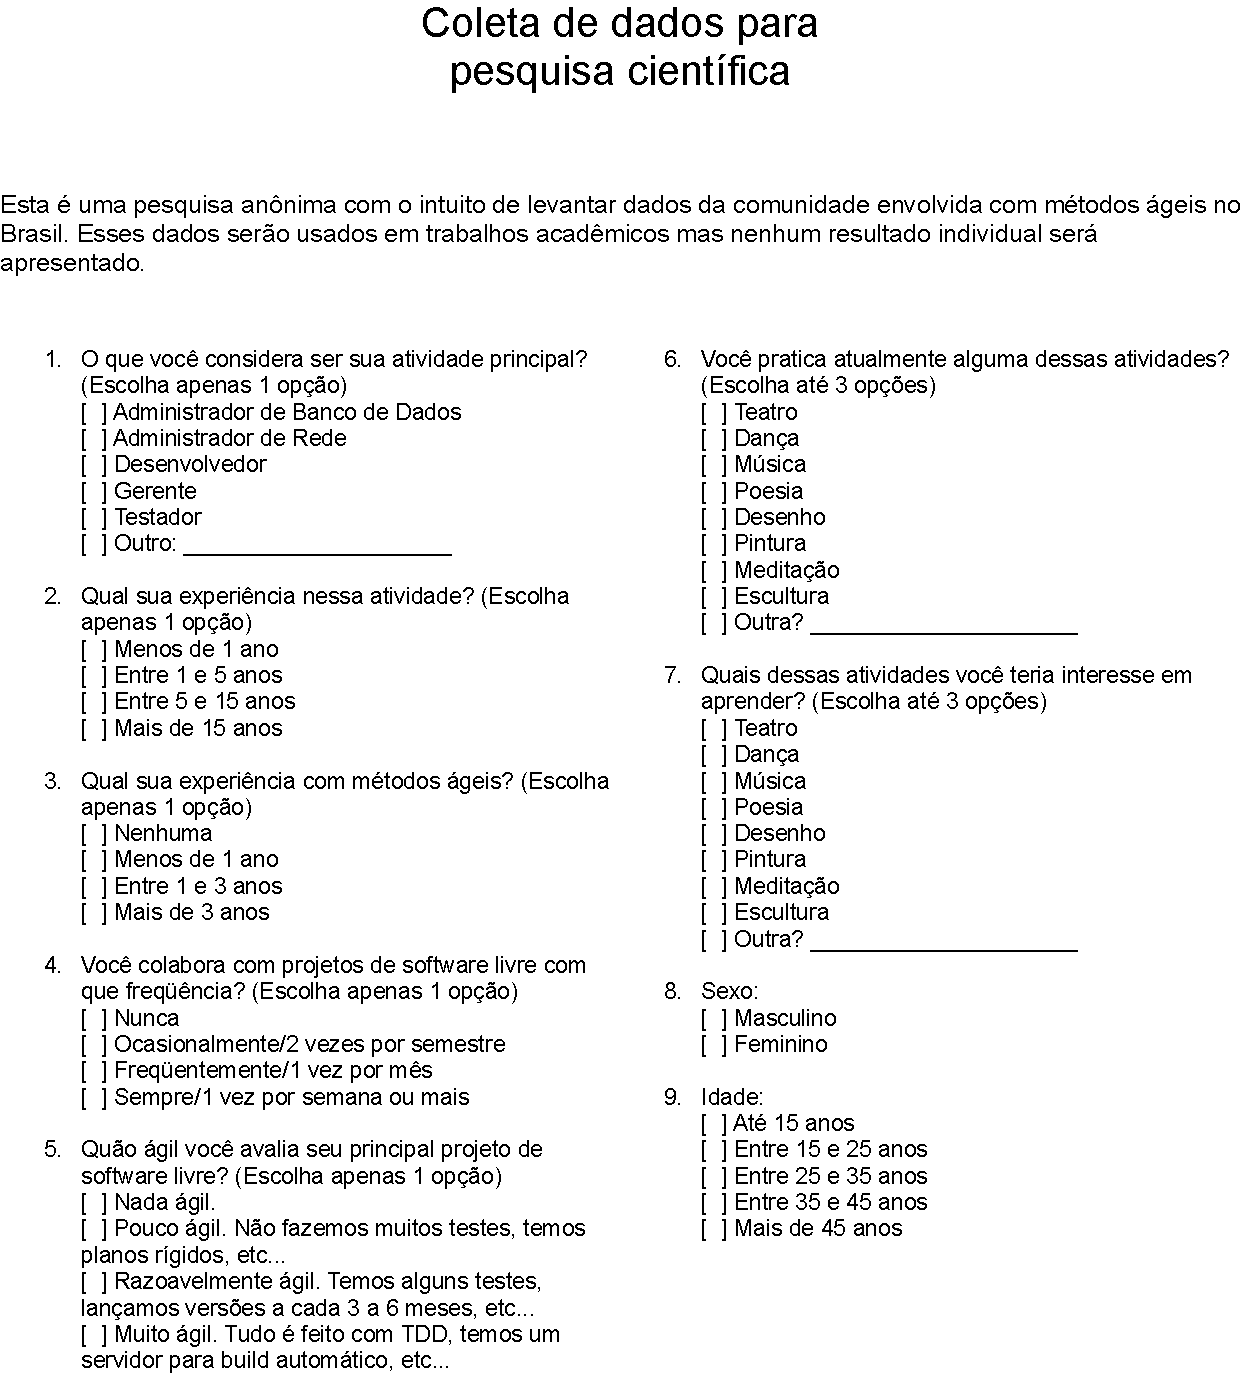
\includegraphics[width=1.0\textwidth]{pesquisaEA}
  \caption{Conteúdo da pesquisa do Encontro Ágil}
  \label{fig:pesquisaEA}
\end{figure}

As respostas foram coletadas ao final do evento quando os
participantes deixavam os formulários na mesa disponível na saída. Os
resultados coletados interessantes no contexto desse trabalho foram os
seguintes:

\begin{enumerate}
\item O que você considera ser sua atividade principal?
  \begin{itemize}
  \item Administrador de Banco de Dados: 1,08\% (1)
  \item Administrador de Rede: 3,23\% (3)
  \item Desenvolvedor: 58,06\% (54)
  \item Gerente: 26,88\% (25)
  \item Testador: 3,23\% (3)
  \item Analista: 3,23\% (3)
  \item Acadêmico: 2,15\% (2)
  \item Documentador: 1,08\% (1)
  \item Consultor: 1,08\% (1)
  \end{itemize}

\item Qual sua experiência nessa atividade?
  \begin{itemize}
  \item Menos de 1 ano: 16,13\% (15)
  \item Entre 1 e 5 anos: 50,54\% (47)
  \item Entre 5 e 15 anos: 26,88\% (25)
  \item Mais de 15 anos: 6,45\% (6)
  \end{itemize}

\item Qual sua experiência com métodos ágeis?
  \begin{itemize}
  \item Nenhuma: 40,86\% (38)
  \item Menos de 1 ano: 41,94\% (39)
  \item Entre 1 e 3 anos: 15,05\% (14)
  \item Mais de 3 anos: 2,15\% (2)
  \end{itemize}

\item Você colabora com projetos de software livre com frequência?
  \begin{itemize}
  \item Nunca: 67,74\% (63)
  \item Ocasionalmente/2 vezes por semestre: 24,73\% (23)
  \item Frequentemente/1 vez por mês: 2,15\% (2)
  \item Sempre/1 vez por semana ou mais: 5,38\% (5)
  \end{itemize}

\item Quão ágil você avalia seu principal projeto de software livre?
  (Foram desconsideradas as respostas daqueles que responderam
  ``Nunca'' na pergunta anterior)
  \begin{itemize}
  \item Nada ágil: 31,03\% (9)
  \item Pouco ágil. Não fazemos muitos testes, temos planos rígidos,
    etc...: 24,14\% (7)
  \item Razoavelmente ágil. Temos alguns testes, lançamos versões a
    cada 3 a 6 meses, etc...: 34,48\% (10)
  \item Muito ágil. Tudo é feito com TDD, temos um servidor para build
    automático, etc...: 10,34\% (3)
  \end{itemize}

\item Sexo
  \begin{itemize}
  \item Masculino: 83,87\% (78)
  \item Feminino: 16,13\% (15)
  \end{itemize}

\item Idade
  \begin{itemize}
  \item Entre 15 e 25 anos: 30,11\% (28)
  \item Entre 25 e 35 anos: 52,69\% (49)
  \item Entre 35 e 45 anos: 13,98\% (13)
  \item Mais de 45 anos: 3,23\% (3)
  \end{itemize}
\end{enumerate}
      % associado ao arquivo: 'ape-pesquisaEA.tex'
\chapter{Pesquisa para colaboradores de software livre}
\label{ape:OS}

\singlespacing

A pesquisa abaixo é uma versão traduzida para o Português e adaptada
para impressão da pesquisa disponibilizada em
\url{http://www.ime.usp.br/~corbucci/floss-survey.html} do dia 28 de
Julho de 2009 até o dia 1$^o$ de Novembro de 2009.

\begin{enumerate}
\item País de residência: \verb=_________________=

\item Ano de nascimento: \verb=______=

\item Número de projetos livres com os quais já contribuiu:
  \verb=____=

\item Ano da primeira contribuição num projeto livre: \verb=______=

\item Nome do principal projeto livre para o qual contribui (ou
  contribuiu): \verb= ______________=

\item Ano da primeira contribuição para esse projeto: \verb=______=

\item Principal papel (escolha apenas 1) nesse projeto:
  \begin{itemize}
  \item[( )] Mantenedor
  \item[( )] \textit{Commiter}
  \item[( )] Programador
  \item[( )] Testador
  \item[( )] Documentador
  \item[( )] Relator de bugs/Descritor de requisitos
  \item[( )] Usuário
  \item[( )] Outro: \verb=_________________=
  \end{itemize}

\item Recebe (ou recebeu) algum rendimento por suas contribuições em
  projetos livres?
  \begin{itemize}
  \item[( )] Sim
  \item[( )] Não
  \end{itemize}

\item Se sim, é (ou foi) sua principal fonte de rendimentos?
  \begin{itemize}
  \item[( )] Sim
  \item[( )] Não
  \end{itemize}

\item Se não em alguma das duas anteriores, sua principal fonte de
  renda está ligada com Tecnologia da Informação?
  \begin{itemize}
  \item[( )] Sim
  \item[( )] Não
  \end{itemize}

\item Quantas pessoas trabalham (ou trabalhavam) com você (escolha
  apenas 1) no seu principal projeto livre?
  \begin{itemize}
  \item[( )] 0
  \item[( )] 1 a 5
  \item[( )] 6 a 10
  \item[( )] 11 a 50
  \item[( )] Mais de 50
  \end{itemize}

\item Qual é (ou foi) o principal canal de comunicação (escolha apenas
  1) entre essa equipe?
  \begin{itemize}
  \item[( )] Face a face
  \item[( )] Site na Internet
  \item[( )] Lista de correio eletrônico
  \item[( )] Ferramenta de rastreamento de problemas
  \item[( )] IRC (\textit{Internet Relay Chat} ou Papo Retransmitido
    pela Internet)
  \item[( )] Mensagens Instantâneas
  \item[( )] Correios eletrônicos individuais
  \item[( )] Voz sobre IP (Skype, Ekiga, iChat, etc...)
  \item[( )] Nenhum
  \item[( )] Outro: \verb=_____________=
  \end{itemize}

\item Como você avalia a qualidade de communicação da equipe?

  Péssima \verb=---------------------------------------= Ótima

\item Qual é (ou foi) o principal canal de comunicação (escolha apenas
  1) entre a equipe e os usuários?
  \begin{itemize}
  \item[( )] Face a face
  \item[( )] Site na Internet
  \item[( )] Lista de correio eletrônico
  \item[( )] Ferramenta de rastreamento de problemas
  \item[( )] IRC (\textit{Internet Relay Chat} ou Papo Retransmitido
    pela Internet)
  \item[( )] Mensagens Instantâneas
  \item[( )] Correios eletrônicos individuais
  \item[( )] Voz sobre IP (Skype, Ekiga, iChat, etc...)
  \item[( )] Nenhum
  \item[( )] Outro: \verb=_____________=
  \end{itemize}

\item Como você avalia a qualidade de communicação entre a equipe e os
  usuários?

  Péssima \verb=---------------------------------------= Ótima

\item Quanto esforço você investe (ou investiu) para manter as
  informações do projeto atualizadas?

  Nenhum \verb=---------------------------------------= Enorme

\item Quais das seguintes ferramentas seus projeto já utiliza? Marque
  todas que já utiliza ou utilizou.
  \begin{itemize}
  \item[( )] Mensagem ou Correio Eletrônico automático em caso de
    falha na montagem automática do projeto
  \item[( )] Estado dinâmico da versão em desenvolvimento a partir da
    ferramenta de rastreamento de problemas
  \item[( )] Gerenciamento da ferramenta de rastreamento de problemas
    a partir dos logs de commit do repositório de código
  \item[( )] Lançamento de nova versão a partir de um click no site do
    projeto
  \item[( )] Geração e atualização automática de gráficos de métricas
    a partir do repositório de código
  \item[( )] Ordenação colaborativa da prioridade dos problemas a
    serem endereçados pela equipe de desenvolvimento
  \item[( )] Linha do tempo no site do projeto ligada ao repositório
    de forma a facilitar análises em retrospectivas
  \item[( )] Um robô nos canais de communicação da equipe facilitar a
    comunicação assíncrona
  \end{itemize}

\item Ordene as seguintes ferramentas da que mais reduz (ou reduziria)
  o esforço gasto em comunicação no seu projeto para a que menos reduz
  (ou reduziria). Dê uma nota de 1 a 8 sendo que 1 é a ferramenta mais
  importante e 8 é a menos importante.
  \begin{itemize}
  \item[( )] Mensagem ou Correio Eletrônico automático em caso de
    falha na montagem automática do projeto
  \item[( )] Estado dinâmico da versão em desenvolvimento a partir da
    ferramenta de rastreamento de problemas
  \item[( )] Gerenciamento da ferramenta de rastreamento de problemas
    a partir dos logs de commit do repositório de código
  \item[( )] Lançamento de nova versão a partir de um click no site do
    projeto
  \item[( )] Geração e atualização automática de gráficos de métricas
    a partir do repositório de código
  \item[( )] Ordenação colaborativa da prioridade dos problemas a
    serem endereçados pela equipe de desenvolvimento
  \item[( )] Linha do tempo no site do projeto ligada ao repositório
    de forma a facilitar análises em retrospectivas
  \item[( )] Um robô nos canais de communicação da equipe de forma a
    facilitar a comunicação assíncrona
  \end{itemize}
\end{enumerate}
      % associado ao arquivo: 'ape-pesquisaOS.tex'
\chapter{Pesquisa para praticantes de Métodos Ágeis}
\label{ape:MA}

\singlespacing

A pesquisa abaixo é uma versão em Português para impressão da pesquisa
disponibilizada em
\url{http://www.ime.usp.br/~corbucci/agile-survey.html} do dia 28 de
Julho de 2009 até o dia 28 de Outubro de 2009.

\begin{enumerate}
\item País de moradia: \verb=_________________=

\item Ano de nascimento: \verb=______=

\item Número de projetos que usavam princípios ágeis que participou:
  \begin{itemize}
  \item[( )] 0
  \item[( )] 1 a 5
  \item[( )] 6 a 10
  \item[( )] 11 a 50
  \item[( )] 51 a 100
  \item[( )] Mais de 100
  \end{itemize}

\item Ano do primeiro projeto que usava princípios ágeis que
  participou: \verb=______=

\item Qual é seu principal papel nos projetos ágeis em que participa?
  \begin{itemize}
  \item[( )] Gerente de projeto
  \item[( )] Líder de equipe
  \item[( )] Programador
  \item[( )] Analista de Qualidade
  \item[( )] Testador
  \item[( )] Acompanhador
  \item[( )] Documentador
  \item[( )] Outro: \verb=_________________=
  \end{itemize}

\item Qual número médio de integrantes nas equipes dos projetos ágeis
  que participou?
  \begin{itemize}
  \item[( )] 1 a 5
  \item[( )] 6 a 10
  \item[( )] 11 a 20
  \item[( )] 21 a 50
  \item[( )] 51 a 100
  \item[( )] Mais de 100
  \end{itemize}

\item Já trabalhou em projetos ágeis com uma equipe (ou parte dela)
  distribuída?
  \begin{itemize}
  \item[( )] Sim
  \item[( )] Não
  \end{itemize}

\item Qual é (ou foi) o principal canal de comunicação entre essa
  equipe?
  \begin{itemize}
  \item[( )] Cara a cara
  \item[( )] Site na Internet
  \item[( )] Lista de correio eletrônico
  \item[( )] Ferramenta de rastreamento de problemas
  \item[( )] IRC (Internet Relay Chat)
  \item[( )] Mensagens Instantâneas
  \item[( )] Correios eletrônicos individuais
  \item[( )] Voz sobre IP (Skype, Ekiga, iChat, etc...)
  \item[( )] Nenhum
  \item[( )] Outro: \verb=_____________=
  \end{itemize}

\item Como você avalia a qualidade de communicação da equipe?

  Péssima \verb=---------------------------------------= Ótima

\item Qual é o principal canal de comunicação entre as equipes de seus
  projetos ágeis e os clientes desses projetos?
  \begin{itemize}
  \item[( )] Cara a cara
  \item[( )] Site na Internet
  \item[( )] Lista de correio eletrônico
  \item[( )] Ferramenta de rastreamento de problemas
  \item[( )] IRC (Internet Relay Chat)
  \item[( )] Mensagens Instantâneas
  \item[( )] Correios eletrônicos individuais
  \item[( )] Voz sobre IP (Skype, Ekiga, iChat, etc...)
  \item[( )] Nenhum
  \item[( )] Outro: \verb=_____________=
  \end{itemize}

\item Como você avalia a qualidade de communicação entre essa equipe e
  o cliente?

  Péssima \verb=---------------------------------------= Ótima

\item Ordene os seguintes problemas do que mais atrapalha (ou
  atrapalhava) no seu projeto ágil distribuído ao que menos
  atrapalha (ou atrapalhava)?
  \begin{itemize}
  \item[( )] Descobrir o que os usuários precisavam
  \item[( )] Descobrir qual era a próxima tarefa a ser realizada
  \item[( )] Entender como o projeto funciona do ponto de vista técnico
  \item[( )] Descobrir o estado atual do projeto
  \item[( )] Integrar código no repositório central
  \item[( )] Manter as informações sobre o projeto atualizadas no
    principal canal de comunicação
  \item[( )] Avaliar o trabalho realizado para identificar pontos de
    melhora
  \item[( )] Sincronizar com os outros colaboradores para atingir um
    objetivo comum
  \end{itemize}

\item Ordene as seguintes ferramentas daquela que mais resolveria os
  problemas citados anteriormente para a que menos resolveria.
  \begin{itemize}
  \item[( )] Mensagem ou Correio Eletrônico automático em caso de
    falha na montagem automática do projeto
  \item[( )] Estado dinâmico da versão em desenvolvimento a partir da
    ferramenta de controle de problemas
  \item[( )] Gerenciamento da ferramenta de controle de problemas a
    partir dos logs de commit do repositório de código
  \item[( )] Lançamento de nova versão a partir de um click no site do
    projeto
  \item[( )] Geração e atualização automática de gráficos de métricas
    a partir do repositório de código
  \item[( )] Ordenação colaborativa da prioridade dos problemas a
    serem endereçados pela equipe de desenvolvimento
  \item[( )] Linha do tempo no site do projeto ligada ao repositório
    de forma a facilitar análises em retrospectivas
  \item[( )] Um robô nos canais de communicação da equipe de forma a
    facilitar a comunicação assíncrona
  \end{itemize}

\item Você já contribuiu com projetos de software livre?
  \begin{itemize}
  \item[( )] Sim
  \item[( )] Não
  \end{itemize}

\item Quão ágil você avaliaria o principal projeto de software livre
  com o qual você contribui (ou contribuiu)?

  Nada ágil \verb=---------------------------------------= Muito ágil

\item Ordene os seguintes problemas do que mais atrapalha (ou
  atrapalhava) no seu projeto de software livre ao que menos
  atrapalha (ou atrapalhava)?
  \begin{itemize}
  \item[( )] Descobrir o que os usuários precisavam
  \item[( )] Descobrir qual era a próxima tarefa a ser realizada
  \item[( )] Entender como o projeto funciona do ponto de vista técnico
  \item[( )] Descobrir o estado atual do projeto
  \item[( )] Integrar código no repositório central
  \item[( )] Manter as informações sobre o projeto atualizadas no
    principal canal de comunicação
  \item[( )] Avaliar o trabalho realizado para identificar pontos de
    melhora
  \item[( )] Sincronizar com os outros colaboradores para atingir um
    objetivo comum
  \end{itemize}

\item Ordene as seguintes ferramentas daquela que mais resolveria os
  problemas citados anteriormente para a que menos resolveria.
  \begin{itemize}
  \item[( )] Mensagem ou Correio Eletrônico automático em caso de
    falha na montagem automática do projeto
  \item[( )] Estado dinâmico da versão em desenvolvimento a partir da
    ferramenta de controle de problemas
  \item[( )] Gerenciamento da ferramenta de controle de problemas a
    partir dos logs de commit do repositório de código
  \item[( )] Lançamento de nova versão a partir de um click no site do
    projeto
  \item[( )] Geração e atualização automática de gráficos de métricas
    a partir do repositório de código
  \item[( )] Ordenação colaborativa da prioridade dos problemas a
    serem endereçados pela equipe de desenvolvimento
  \item[( )] Linha do tempo no site do projeto ligada ao repositório
    de forma a facilitar análises em retrospectivas
  \item[( )] Um robô nos canais de communicação da equipe de forma a
    facilitar a comunicação assíncrona
  \end{itemize}
\end{enumerate}
      % associado ao arquivo: 'ape-pesquisaMA.tex'

% ---------------------------------------------------------------------------- %
% Bibliografia
\backmatter \singlespacing   % espaçamento simples

\bibliographystyle{alpha-ime}% citação bibliográfica alpha
\bibliography{bibliografia}  % associado ao arquivo: 'bibliografia.bib'

% ---------------------------------------------------------------------------- %
% Índice remissivo
%\index{TBP|see{periodicidade região codificante}}

%\printindex   % imprime o índice remissivo no documento 

\end{document}

